\section*{Introduction}
Welcome to the practicals for EEE3096S. These instruction are applicable to all practicals so please take note.

All files submitted to Vula must be in the format Studnm\_pracnum.fileformat

All reports must be done in Latex. Marks will be deducted if they are not.

It is critical to do the pre-prac work. Tutors will not help you with questions with answers that would have been known had you done the pre-prac work. 

The practical handbook introduces the important tools, knowledge and skills you will need for these practicals. While references to more detailed information is given, students are encouraged to learn more about these topics using the internet and to take responsibility for their learning.

\newpage
\setcounter{section}{-1}
\section{Prac 0 - Setting up and Connecting to Your Pi}
The Raspberry Pi is a powerful SBC. While it can be used as a lightweight computer, its true strengths come from how versatile the platform is\footnote{Some examples include \href{https://www.home-assistant.io/hassio/}{home automation}, \href{https://xbian.org/getting-started/}{media centre} or even as a \href{https://github.com/takyonxxx/BalanceRobot-Raspberry-Pi}{robot}}.  We will be using the Pi throughout the rest of the course in both practicals and the mini project.  Before you attend the first tutorial session is is required that you setup your Pi so it is ready for operation.  In addition, if you are unfamiliar with Linux, Git, ssh, and bash we strongly recommend you go through the additional exercises as outlined in the lab handbook.

\subsection{Required before attending the first lab session: Setup your Pi }
Before arriving at the first practical lab session of this course you are required to do the following. If you have trouble completing the following you should attend the hotseat on \textbf{Friday the 19th of July} to get help before the first lab session.
\begin{enumerate}
    \item Setup your Pi and get SSH working, as per the lab handbook.
    \item Create a GitHub account, and sign up for the \href{https://education.github.com/pack}{GitHub Education Pack}.
    \item Enable Ethernet pass-through on the Pi to give it internet access. Instructions can be found in the lab handbook.
    \item Fetch the practical repository
    \begin{enumerate}
        \item SSH in to the Pi
        \item Ensure you have connectivity by trying to ping a website such as google.com. If not, debug your connection.
        \item Fetch the repository
            \begin{lstlisting}[gobble=12]
            $ git clone --depth=1 https://github.com/kcranky/EEE3096S.git PracSource/
            \end{lstlisting}
        \item Create a copy of the original git folder
            \begin{lstlisting}[gobble=12]
            $ mkdir mypracs
            $ cp -r PracSource mypracs
            \end{lstlisting}
        \item Remove the git settings
            \begin{lstlisting}[gobble=12]
            $ cd mypracs
            $ rm -rf .git
            \end{lstlisting}
        \item Initialise a new repository, and put it on GitHub as per the instructions in "A Quick Git Get Go" in the lab handbook.
    \end{enumerate}
\end{enumerate}

\subsection{Submissions}
There are no submissions for this practical.


\newpage
\section{Practical 1 - Git, Bash, GPIO}
\label{sec:Prac1}
\subsection{Overview}
This practical sets out to familiarise you with the Pi and complete a simple programming task. If you have not yet done so, complete Prac 0. Ensure that you can SSH into the pi, as all the tasks for this prac require it.

To be completed individually. 

\textbf{Due date:} See Vula

\subsection{Pre-Prac Tasks}
\begin{itemize}
\itemsep0em 
    \item Complete Prac 0 to have your Pi set up and configured
    \item Read the sections "Inputs" and "Outputs" on the RPi.GPIO documentation, available \href{https://sourceforge.net/p/raspberry-gpio-python/wiki/Examples/}{here}
    \item Update your pracsource git repository, as there has been an update to the Python template
\end{itemize}

\subsection{Pre-prac Requirements}
This section covers what you will need to know before starting the practical.
\begin{itemize}
    \itemsep0em 
    \item Have your Raspberry Pi Set up as per the requirements of Prac 0.
    \item Have an understanding of how you can edit text files on the Pi using an editor such as nano, or using VNC and a GUI-based editor.
    \item Have a basic understanding of Git
\end{itemize}

\subsection{Hardware Required}
\begin{table}[H]
\begin{tabular}{ll}
\begin{tabular}[c]{@{}l@{}}\tabitem Raspberry Pi with configured SD Card\\ \tabitem RPi Power Supply\\ \tabitem Ethernet Cable\\ \tabitem A breadboard \end{tabular} & \begin{tabular}[c]{@{}l@{}}\tabitem 2 x push buttons\\ \tabitem 3 x LEDs\\ \tabitem 3 x Resistors\\ \tabitem Dupont Wires\\\end{tabular} \\
\end{tabular}%
\end{table}

\subsection{Outcomes of this Practical}
You will learn about the following topics:
\begin{table}[H]
\begin{tabular}[c]{@{}l@{}}\tabitem Basic GPIO Usage\\ \tabitem Interrupts\\ \tabitem Debouncing \end{tabular}
\begin{tabular}[c]{@{}l@{}}\tabitem Git\\ \tabitem Bash\\ \tabitem SSH\\ \end{tabular}  
\end{table}

\subsection{Deliverables}
At the end of this practical, you must:
\begin{itemize}
\itemsep0em 
    \item Demonstrate your working implementation of the binary counter to a tutor
    \item Single PDF with your screenshots from the Terminal task to Vula in a pdf document. This PDF document should also contain a link to your GitHub repository. 
\end{itemize}

\subsection{Walkthrough}
This practical consists of two parts. The terminal task can be completed at home and does not require demonstration to a tutor.

\subsubsection{Terminal Task}
\label{sec:Prac1:Terminal}
While there are many Graphic User Interfaces (GUI) available for various distributions of Linux including Raspbian, it is often necessary to operate an embedded system without a GUI given the limited processing and memory resources of the device.  Consequently it is important to learn to use Linux through the command line shell. A very common shell on many Linux systems is Bash.  Learning about and being comfortable with the command line will help you greatly in working with embedded systems.  The tasks below will introduce basics to you, but you should consult the manual for more information.

Start by SSH'ing into your Pi and create a folder called \textless your\_student\_number\textgreater.\\
Run the following commands, and take a screenshot after each command:
\begin{itemize}
\itemsep0em 
    \item \$ ls (must show the folder you just created)
    \item \$ ifconfig (eth0 must be visible)
    \item \$ lscpu (number of cores must be visible)
\end{itemize}
Your result should look something like this:
\begin{figure}[H]
\centering
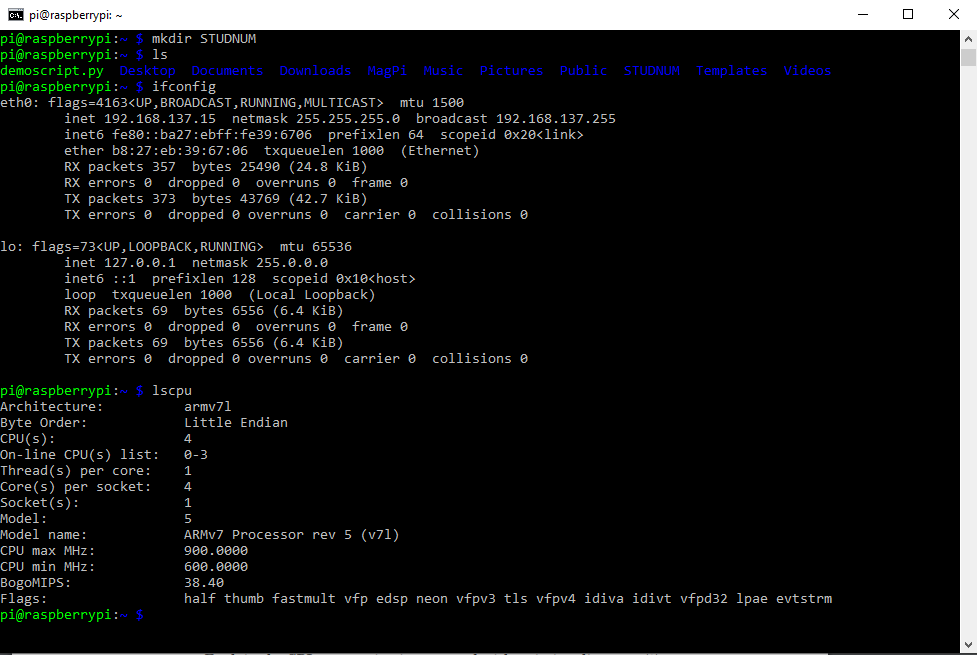
\includegraphics[width=0.6\columnwidth]{Figures/CMDOutput}
\caption{Example output after running the above commands}
\label{fig:CMDOutput}
\end{figure}



\subsubsection{Programming Task}
In this task you will develop a simple 3-bit binary counter, the values of which will be placed on LEDs connected to the Pi. The value on the counter should change depending on a button press.
Be sure to use git to keep track of changes to your code. For instructions on using Git, refer to the lab handbook.
\begin{itemize}
\itemsep0em 
    \item Start by connecting to your Pi through VNC or SSH (see lab handbook)
    \item If not installed, install the Python GPIO libraries, as explained \href{https://pythonhosted.org/RPIO/}{here}. (They should be installed by default.)
    \item Connect 3 LEDs and 2 Push buttons to the GPIO pins of the Pi - taking care of which pins to use. Look at \href{pinout.xyz}{pinout.xyz} and be sure to not use special purpose pins
    \item Read the Python Tips and tricks in the lab handbook to gain understanding of the commands and why they are used.
    \item Create a copy of the template in the mypracs folder.
    \item Write your code. It's suggested you work incrementally, committing your code using git each time you accomplish something. 
    \begin{itemize}
    \itemsep0em 
        \item Take a look at the RPI.GPIO examples, available \href{https://sourceforge.net/p/raspberry-gpio-python/wiki/Examples/}{here}
        \item Start by turning on and off a single LED in the main() method. Delay between toggling the GPIO by using something like \verb|time.sleep()|
        \item Now, use a button to toggle the state of the LED. Look at the lab handbook for help with debouncing and interrupts in Python.
        \item Finally, implement a system that displays a binary value on 3 LEDs. Use one button to increase the value, and another button to decrease the value. The values should wrap around (i.e. increasing "111" should then display "000" and decreasing "000" should display "111"
    \end{itemize}
    \item Hints
    \begin{itemize}
    \itemsep0em 
        \item Look at \textit{itertools.product} to generate a list of binary values.
        \item Use a single integer counter as an index to the Python array that you've created. Make use of Python's \verb|global| construct to do so
    \end{itemize}
    \item Demonstrate this implementation to a tutor to get signed off, and push your code to GitHub.
    \item Submit a PDF as per the deliverables section
\end{itemize}

\subsection{Mark Allocations}
Marks will be given for:
\begin{itemize}
\itemsep0em 
    \item Correctly completing the terminal task
    \item Well structured and commented code
    \item Meaningful git commit messages
    \item A correct demonstration
\end{itemize}
Marks will be deducted for:
\begin{itemize}
\itemsep0em 
    \item Not using interrupts and debouncing on your button presses
    \item Not submitting files in the correct format
    \item Not linking to the practical on GitHub
    \item Copying another student's code
    \item Late submission
\end{itemize}
\newpage
\section{Prac 2 - Python vs. C}
\label{sec:Prac2}

\subsection{Overview}
This practical will show you the importance of C for embedded systems development. 

\subsection{Pre-prac Requirements}
This section covers what you will need to know before starting the practical.
\begin{itemize}
    \item Cross compilation
    \item Makefiles
    \item Introduction to benchmarking concepts (not looking at only one benchmark, hot boards, etc)
    \item Introduction to cache warming and good testing methodology (multiple runs, wall clock time, speed up)
\end{itemize}

\subsection{Outcomes}
You will learn about the following aspects:
\begin{itemize}
    \item Heterodyning
    \item Benchmarking
    \item Latex
    \item Bit widths (too much?)
    \item Compiler flags (too much?)
    \item Instruction sets (will be required for floating and compiler flags eg \$cat /proc/cpuinfo)
\end{itemize}

\subsection{Deliverables}
At the end of this practical, you must:
\begin{itemize}
    \item Submit a 3 page report in IEEE-Conference style detailing your investigation
\end{itemize}

\subsection{Hardware Required}
\begin{itemize}
    \item Raspberry Pi
    \item SD Card
    \item Ethernet Cable
\end{itemize}

\subsection{Further Instructions}
\textbf{Instructions to tutors:}
\begin{itemize}
    \item Further develop the prac overview to give a short blurb on heterodyning (it's use, etc)
    \item Develop C and Python code for heterodyning
    \item Include the guides for cross compilation as listed in the appendix
    \item Decide on an independent variable for testing the implementation (bit width maybe? 16 vs 32 vs 64 bit floating point by setting C compiler flags? Or decide if just testing C and python is enough)
    \item Write up the walkthrough section of this practical and adapt any other sections of this prac
    \item Link to Overleaf and a guide on how to get the IEEE conference template (new project -\textgreater  from template -\textgreater  etc)
\end{itemize}


Not sure if the following  is too much but I've included it anyway in case the tutors decide it's doable given the nature of the prac:\\
Prac 2 should be be a mathematical benchmark comparison, using floating vs fixed point math, dealing with compiler optimizations for C and hardware level support for the RPi. Students are also exposed to instruction sets (\$cat /proc/cpuinfo), compiler flags (-mfp16-format=ieee, setting HW floating point compiler directives such as fpv4, vfpv3, vfpv3xd, etc).


\newpage
\section{Prac 3 - SPI and Threading}
\label{sec:Prac3}
\subsection{Overview}
While the Pi does have an audio jack, it uses a purely PWM (pulse width modulation) based implementation for audio. Audiophiles among you may know that this is not a great way of playing audio. You can read more about the Raspberry Pi and it's audio jack \href{https://hackaday.com/2018/07/13/behind-the-pin-how-the-raspberry-pi-gets-its-audio/}{here}.

To improve audio quality, we can use a DAC (digital to analog converter). In this practical, you will pass sampled audio data over SPI to a 10 bit DAC for playback. 

\subsection{Pre-prac requirements}
This section covers what you will need to know before starting the practical.
\begin{itemize}
    \item Interrupts
\end{itemize}

\subsection{Outcomes}
You will learn about the following aspects:
\begin{itemize}
    \item SPI
    \item Threading
\end{itemize}

\subsection{Deliverables}
At the end of this practical, you must:
\begin{itemize}
    \item Demonstrate your working implementation to a tutor
    \item Submit your code on Vula
\end{itemize}

\subsection{Hardware Required}
\begin{itemize}
    \item Raspberry Pi
    \item SD Card
    \item Ethernet Cable
    \item Breadboard
    \item Jumper wires
    \item X x Buttons (Depends on number of samples)
    \item MCP4911 DAC Chip
    \item Speaker to play sound (Supplied by lab?)
\end{itemize}


\subsection{Further Instructions}
\textbf{Instructions to tutors:}
\begin{itemize}
    \item Flesh out all the sections in the guide
    \item Complete this practical and write instructions for students
    \item You must be able to press a button to play audio. 
    \item Transfer to the DAC should happen on a second thread
    \item If something is playing and another button is pressed, the new audio should be played (ie the current playing audio should be replaced by the new file)
\end{itemize}
\newpage
\section{Prac 4 - I2C and PWM}
\label{sec:Prac4}
\subsection{Overview}
Something about why loading scripts on Pi on startup is useful. Something about RTCs and why they are useful (especially considering the Pi doesn't have one)

\subsection{Pre-prac requirements}
This section covers what you will need to know before starting the practical.
\begin{itemize}
    \item I2C
    \item PWM
    \item Knowledge about BASH as learnt in previous pracs
\end{itemize}

\subsection{Outcomes}
You will learn about the following aspects:
\begin{itemize}
    \item I2C
    \item Real Time Clocks
    \item Starting a script on boot on the Raspberry Pi
\end{itemize}

\subsection{Deliverables}
At the end of this practical, you must:
\begin{itemize}
    \item Demonstrate your working implementation to a tutor
    \item Submit your code on Vula
\end{itemize}

\subsection{Hardware Required}
\begin{itemize}
    \item Raspberry Pi
    \item SD Card
    \item Ethernet Cable
    \item Breadboard
    \item Jumper wires
    \item 2 x Buttons
    \item RTC
    \item 11 LEDs (4 for hours, 6 for minutes, 1 for seconds)
    \item 11 Resistors for said LEDs
\end{itemize}


\subsection{Further Instructions}
\textbf{Instructions to tutors:}
\begin{itemize}
    \item Flesh out all the sections in the guide
    \item Complete this practical and write instructions for students
    \item The time from the RTC should be displayed in binary format on the LEDs
    \item The "seconds" LED should be at it's dimmest when the minute starts, and at it's brightest just before the minutes value increases (ie it should be min brightness at 0 seconds, and max brightness at 59.99 seconds)
    \item One button should increase the hours value, another button increase the minutes value
\end{itemize}
\newpage
\section{Prac 5 - ALU}
\label{sec:Prac5}
\subsection{Overview}
An arithmetic logic unit (ALU) is a digital building block which can perform a variety of arithmetic, logical and bit shift operations. It is the base building block of a central processing unit and operates on integer binary numbers. The unit has both data and control signals. A basic ALU has two parallel input data busses (A) and (B) and one parallel output data bus (Y). It also has a parallel bus (F) which takes in an opcode or binary value which selects a specific arithmetic, logical or shift operation to be performed by the ALU on the two inputs A and B, it may also have a status output bus S which gives more information about the previous operation.
\begin{figure}[H]
\centering
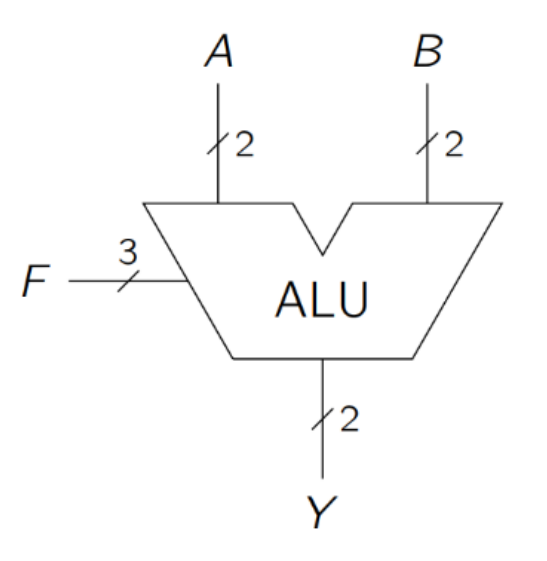
\includegraphics[width=0.35\columnwidth]{Figures/ALU}
\caption{An Example of a simple ALU with a 2-bit wide data bus}
\label{fig:ALU}
\end{figure}

\subsection{Pre-Practical Requirements}
\begin{itemize}
    \item Logisim
    \item Latex
\end{itemize}

\subsection{Deliverables}
\begin{itemize}
    \item Design the ALU using logical building blocks. Explain each step in your report. (30) \footnote{This is not a technical report as the one expected in practical 2. However, each building blocks must be represented in a figure, the functionality and the role of each building block in the bigger system must be explained.}
    \item Simulate your design in Logisim. Clearly label all inputs, outputs etc. Export a jpeg of the circuit and include it in your report. (10)
    \item Marks will be deducted for incomplete or untidy reports.
\end{itemize}


\section{Further Instructions}
You are required to design and implement a 2-bit wide ALU with a 3 bit opcode, as follows:
% Please add the following required packages to your document preamble:
% \usepackage{graphicx}
\begin{table}[H]
\centering
\caption{Three bit opcode and equivalent operation}
\label{tbl:Opcodes}
\begin{tabular}{|c|c|c|c|c|}
\hline
\multicolumn{3}{|c|}{\textbf{Opcode}} & \multicolumn{2}{c|}{\textbf{Function}} \\ \hline
$F_2$ & $F_1$ & $F_0$ & \multicolumn{2}{c|}{F} \\ \hline
0 & 0 & 0 & A+B & Addition \\ \hline
0 & 0 & 1 & A-B & Subtration \\ \hline
0 & 1 & 0 & A+1 & Increment \\ \hline
0 & 1 & 1 & A-1 & Decrement \\ \hline
1 & 0 & 0 & A $\times$ 2 & Multiply by 2 \\ \hline
1 & 0 & 1 & A \textdiv 2 & Divide by 2 \\ \hline
1 & 1 & 0 & A $\wedge$ B & Bit-wise AND \\ \hline
1 & 1 & 1 & A $\vee$ B & Bit-wise OR \\ \hline
\end{tabular}%
\end{table}
